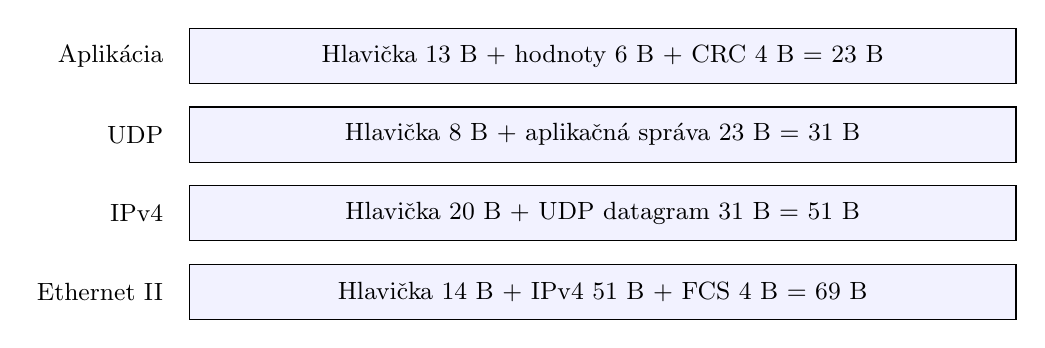
\begin{tikzpicture}[x=1cm,y=1cm,font=\small]
\foreach \y/\label/\content in {0/Aplikácia/{Hlavička 13 B + hodnoty 6 B + CRC 4 B = 23 B},-1/UDP/{Hlavička 8 B + aplikačná správa 23 B = 31 B},-2/IPv4/{Hlavička 20 B + UDP datagram 31 B = 51 B},-3/Ethernet II/{Hlavička 14 B + IPv4 51 B + FCS 4 B = 69 B}} {
 \node[anchor=east] at (1,\y) {\label};
 \node[draw,fill=blue!5,minimum width=10.5cm,minimum height=7mm,anchor=west] at (1.2,\y) {\content};
}
\end{tikzpicture}
